\chapter{Implementacja}

% SW2: Ten rodział powienien rozpoczynać się "wprowadzeniem" do implementacji -- rozpoczynanie opisu od listy katalogów jest dezorientujące. To wprowadzenie powinno przedstawiać -- może nawet w formie grafu -- główne kroki w programie (opisane później szczegółowo w kolejnych podpunktach), wprowadzać terminologię używaną w bardziej szczegółowych opisach (nadal nie wiem, co rozumie Pan przez "terapię" lub "element terapii"), wyjaśniać sposób identyfikowania wierzchołków grafu/elementóW terapii i na końcu wreszcie opisywać źródła danych/wiedzy wykorzystywane przez program (tutaj wreszcie mogą pojawić się katalogi i ich opis).
 
\section{Struktura katalogów}

\begin{itemize}
\item{Algorytmy – zawiera pliki o rozszerzeniu dot opisujące grafy procedur medycznych chorób}
\item{Konflikty – zawiera opisy konfliktów, jakie występują między chorobami oraz zmiany, które należy wprowadzić w przypadku wystąpienia konfliktów}
\item{Grafy – zawiera zmodyfikowane grafy chorób przedstawiające aktualnie przebytą ścieżkę oraz grafy wynikowe prezentujące rozwiązania. Grafy są w dwóch formatach – tekstowym w formacie dot oraz graficznym w formacie png. 
% SW: Rozumiem, że zawartość tego katalogu jest kasowana *podczas* zamykania programu?
Podczas zamykania programu zawartość tego katalogu jest kasowana}
\end{itemize}
\section{Klasy systemu}
\begin{itemize}
\item{AddToTherapy - dodawanie identyfikatorów węzłów do listy opisującej konkretną terapię}
\item{ChocoClass - rozwiązanie problemu CLP}
\item{Color - kolorowanie wierzchołków i krawędzi grafów}
\item{CreateTherapies - generowanie terapii}
\item{ExecuteInteractions - wprowadzanie zmian w terapiach w przypadku wykrycia konfliktów}
\item{GoForward - przechodzenie do kolejnego węzła decyzyjnego}
\item{GraphFunctions - przydatne funkcje związane z grafami, np. znalezienie węzłów docelowych określonego węzła}
\item{ImageGraph - wyświetlanie grafów}
\item{MainClass - obsługa zdarzenia kliknięcia przycisku Dalej}
\item{RadioButtonList - tworzenie i obsługa zdarzeń list pól wyboru służących do udzielania odpowiedzi na pytania}
\item{Results - wyświetlanie wyników}
\item{Window - okno programu}
\end{itemize}

% SW2: W całym tym opisie mówimy o METODACH, a nie o FUNKCJACH (Java jest językiem obiektowym).
\section{Wybór chorób}
% SW2: Opis każdego z istotnych kroków programu warto rozpocząć od krótkiej (1-2 zdania) informacji, co jest jego głównym celem. W tym przypadku celem jest umożliwienie użytkownikowi wyboru tych wytycznych, które będą rozważane dla aktualnego pacjenta.

% SW2: W jakiej klasie/metodzie zrealizowana jest ta funkcjonalność? Taką informację proszę zamieścić dla wszystkich omawianych kroków programu.
W katalogu Algorytmy program szuka plików posiadających rozszerzenie DOT. Dla każdego takiego pliku tworzone jest pole wyboru. Pole wyboru posiada etykietę równą nazwie choroby. 
% SW2: W jakiej klasie znajduje się pole checkBoxGroup? Proszę podać jej szczegółową "lokalizację". Podobna uwaga dotyczy wszystkich tych miejsc, gdzie odwołuje się Pan do pól w różnych klasach.
Utworzone pole wyboru jest następnie dodawane do globalnej listy pól wyboru o nazwie \texttt{checkBoxGroup} oraz do panelu 
znajdującego się w lewym górnym rogu okna programu (rys. \ref{fig:wybor_chorob}). 
\begin{figure}[H]
\centering
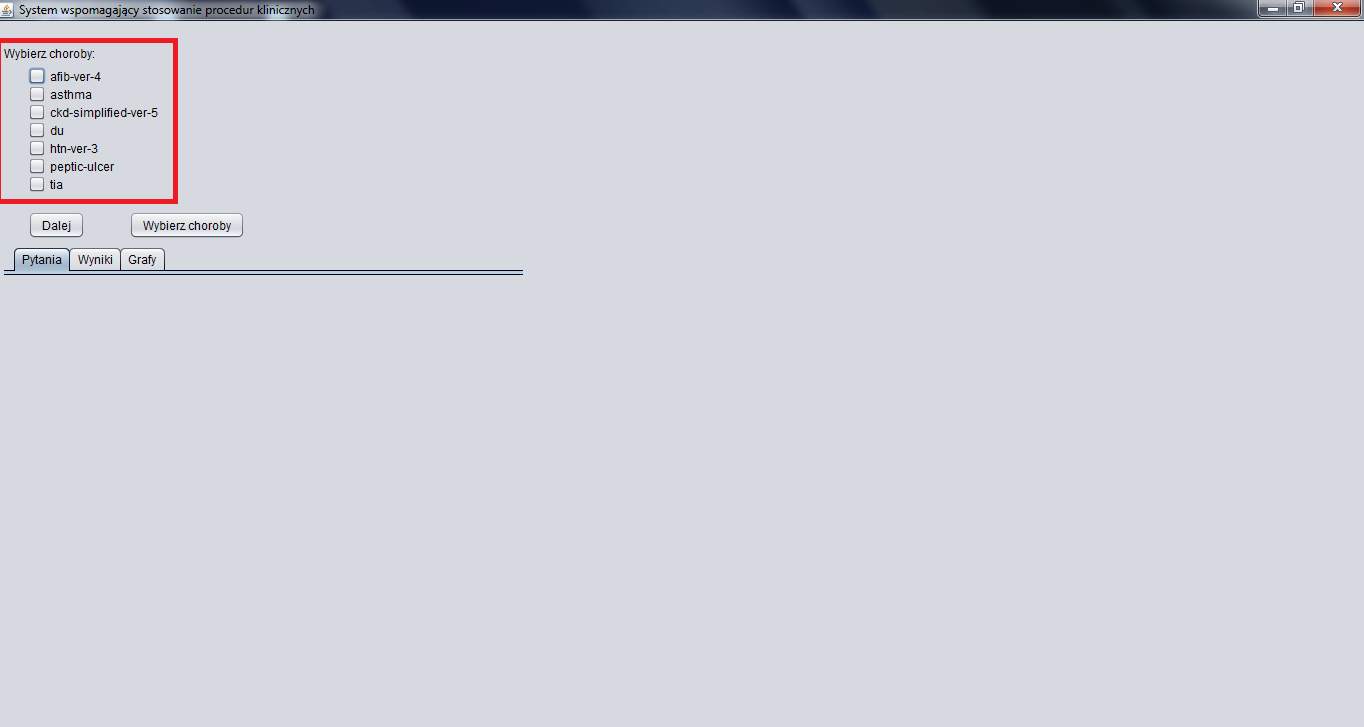
\includegraphics[width=\textwidth]{img/wybor_chorob.png}
% SW2: Każdy rysunek MUSI mieć swój tytuł i numer, a w tekście MUSI się znaleźć do niego odwołanie. Poza tym w tym przypadku rysunek powinien zostać wykadrowany tak, aby ograniczał się przede wszystkim do panelu wyboru. Nie ma potrzeby zamieszczania wielkiego okna ekranu w sytuacji, gdy chcemy zademonstrować tylko jego niewielki fragment.
\caption{Panel wyboru chorób}
\label{fig:wybor_chorob}
\end{figure}
Po wybraniu chorób, tzn. po kliknięciu w odpowiednie pola wyboru i kliknięciu przycisku „Dalej”, nazwy wybranych chorób są dodawane do listy o nazwie \texttt{selectedDiseases} i program przechodzi do fazy wyświetlania grafów. 

\section{Wyświetlanie grafów}

% SW2: Tutaj celem jest stworzenie graficznej reprezentacji wybranych wytycznych. Wytyczne przedstawiane są postaci grafu, w którym zaznaczno odwiedzone wierzchołki i krawędzie (odpowiadające wykonanym akcjom, podjętym wyborom oraz wyborom oczekującym na informację zwrotną od użytkownika).

% SW2: Co to znaczy, że program odczytuje z funkcji graf? To chyba metoda odczytuje graf z pliku i zwraca go do wywołującej metody?
Na początku program odczytuje z funkcji \texttt{GraphFunctions.getGraph} graf znajdujący się w pliku o rozszerzeniu dot oraz pobiera 
% SW2: Węzeł początkowy to korzeń grafu.
węzeł początkowy grafu. Operacje te wykonywane są dla wytycznych związanych z każdą z wybranych chorób. Funkcja \texttt{getGraph} korzysta z funkcji \texttt{parse} obiektu klasy \texttt{Parser} z biblioteki JPGD. 
% SW2: To już napisał Pan wyżej -- proszę unikać powtórzeń
Po odczytaniu grafu za pomocą funkcji \texttt{GraphFunctions.getStartNode} program znajduje węzeł początkowy grafu. Znalezienie takiego węzła polega na wyszukaniu węzła, który nie posiada 
% SW: Tutaj raczej chodzi o krawędź dochodzącą.
krawędzi wejściowej. 

Następnie dla każdej choroby wywoływane są funkcje \texttt{MainClass.execute}, \texttt{ImageGraph.new ImageGraph} oraz \texttt{RadioButtonList.createRadioButtonList}. Pierwsza z nich przemieszcza się po grafie, 
% SW2: Dlaczego przechodzimy tylko do pierwszego kroku? Co w sytuacji, w której wyświetlamy graf, dla którego mamy więcej informacji (np. odpowiedzi na 2-3 początkowe pytania)?
aby odnaleźć pierwszy krok decyzyjny w wytycznych, oraz wywołuje funkcję \texttt{Color.color}, która zaznacza przebytą ścieżkę w grafie. Podczas poruszania się po grafie do listy list o nazwie \texttt{dataIdList} dodawane są identyfikatory węzłów, na które program natrafił. Dzięki \texttt{dataIdList} funkcja \texttt{Color.color} może pokolorować kontury przebytych węzłów oraz przebyte krawędzie, a także je pogrubić. 
% SW: Co to jest "element terapii"? Czy sa to tylko wierzchołki związane z akcjami? To sugerowałoby rozróżnienie między elementem terapii, a węzłem. Nie jest też jasne, czy element terapii to obiekt, czy tylko jego nazwa -- pisze Pan o "częsci elementu terapii przed znakiem zapytania". 

% SW2: Biorąc pod uwagę Pana wyjaśnienie Color to klasa, a nie metoda.
Funkcja \texttt{Color} dla każdego elementu terapii określonej choroby znajdującego się w \texttt{dataIdList} szuka w grafie węzła posiadającego identyfikator o tej samej wartości, co element terapii lub węzła, którego identyfikator jest równy części elementu terapii przed znakiem zapytania. Element terapii to identyfikator węzła w przypadku węzłów akcji, natomiast dla węzłów decyzji elementem terapii są identyfikator węzła i etykieta wybranej krawędzi oddzielone znakiem zapytania.
% SW: Z poniższego opisu wynika, że element terapii to nazwa/identyfikator. To należy jasno na początku wyjaśnić. Również na początku należy wyjaśnić, jak tworzy Pan identyfikatory dla krawędzi wychodzących z węzłów decyzyjnych, aby później było jasne, dlaczego mówimy o części "elementu terapii" przed znakiem zapytania.
% SW2: Czy przez znaznaczanie rozumie Pan zmianę koloru oraz pogrubianie konturu/linii dla węzła lub krawędzi poprzez zmianę odpowiednich atrybutów? Poza tym poniższy opis nie jest chyba zgodny z zachowaniem programu -- jeśli wartość związana z węzłem decyzyjnym nie jest znana, żadna z krawędzy wyjściowych nie jest zaznaczana.
W przypadku, gdy element terapii nie posiada znaku zapytania, zaznaczany jest znaleziony węzeł oraz wszystkie jego krawędzie wyjściowe.  Jeśli element terapii zawiera znak zapytania, zaznaczany jest znaleziony węzeł oraz krawędź, której etykieta jest równa części elementu terapii po znaku zapytania.
 
Po wywołaniu funkcji color wywołana zostaje funkcja \texttt{ImageGraph.newImageGraph}, której zadaniem jest wygenerowanie i wyświetlenie nowego obrazu grafu. Na początku funkcja zapisuje do pliku wynik funkcji \texttt{toString} wywołanej dla grafu (wynik funkcji \texttt{toString} należało poprawić, biblioteka JPGD zawiera drobne błędy). Następnie wywoływana jest funkcja \texttt{ImageGraph.getImageGraphPath}, która uruchamia program DOT i tworzy z zapisanego wcześniej pliku tekstowego graf w postaci obrazu w formacie PNG. W kolejnym kroku funkcja \texttt{ImageGraph.newImageGraph} tworzy obiekt klasy \texttt{BufferedImage} z wygenerowanym w poprzednim kroku obrazem. Później funkcja dokonuje skalowania obrazu tak, aby mógł on się zmieścić na etykiecie. 
% SW: Tutaj lepiej mówić o pewnym progu narzuconym na rozmiar, aby uniknąć (słusznego skądinąd) zarzutu o nieskalowalności intefejsu w programie.
Jeśli szerokość lub wysokość obrazu przekracza próg 900 pikseli, obraz zmniejszany jest do 2/3 wielkości tak, aby był on czytelny (w tym przypadku do etykiety dodawane są suwaki). Ponadto, jeżeli szerokość i wysokość obrazu jest mniejsza od wielkości etykiety, to na etykiecie umieszczany jest obraz bez skalowania, w skali 1:1.
 
Ostatnim krokiem jest wywołanie funkcji \texttt{RadioButtonList.createRadioButtonList}. 
% SW2: Tutaj powinien Pan wyjaśnić, że elementy terapii zawierające znak zapytania odpowiadają krokom decyzyjnym.
Funkcja ta dla każdego elementu terapii, który posiada znak zapytania tworzy panel. Pierwszym elementem panelu jest etykieta węzła. 
% SW: Pola wyboru zamiast "radiobuttonów".
Pozostałe elementy stanowią pola wyboru z etykietami, których wartości są równe etykietom krawędzi węzła decyzyjnego. 
Do tych pól wyboru dodawany jest jeszcze jeden z etykietą „brak wartości”, przydatny w sytuacji, gdy nie znamy jeszcze danych. 
% SW2: Ta część elementu terapii nie tyle pozwala na wybranie jednej z możliwości, ale na przechowanie informacji o wyborze.
Część elementu terapii po znaku zapytania pozwala na wybranie aktywnego pola wyboru. 
% SW: Chwilę wcześniej pisał Pan o tworzeniu pól wyboru dla "braku wartości". Dlaczego to Pan powtarza?
% SW2: Kiedy aktualizowana jest lista lastNodes? Nigdy wcześniej nie wspomina Pan o niej w opisie. Czy jest ona aktualizowana przez MainClass.execute? To należy wyjaśnić.
Na końcu tworzony jest jeszcze jeden panel, tym razem dla pytania, na które jeszcze nie została udzielona odpowiedź, dla niego zaznaczone jest pole wyboru z etykietą „brak wartości”. Panel ten jest związany z węzłem znajdującym się na liście lastNodes. Przy pierwszym wyświetleniu grafu tworzony jest tylko ten panel. Ponadto, dla każdego pola wyboru przypisywane jest zdarzenie \texttt{RadioButtonList.updateRadioButtonList}.
% SW: Myślę, że tutaj pomocne byłoby pokazanie przykładowego ekranu i wskazanie na powiązanie między pytaniami, a aktualną ścieżką w grafie.
 
% SW: Zamiasts opisywać, lepiek pokazać ekran.
Ostatecznie grafy prezentowane są po prawej stronie ekranu na zakładkach. Każda zakładka dotyczy wytycznych związanych z jedną z wybranych chorób. Z lewej strony ekranu pojawiają się natomiast zakładki z listami pól wyboru. W tym przypadku również jedna zakładka dotyczy specyficznych wytycznych. Listy pól wyboru pozwalają na udzielanie odpowiedzi na pytania zawarte w wytycznych klinicznych. 
% SW2: Do rysunku odwołujemy się przez podanie jego numeru
Przykład wyświetlanych grafów przedstawiono na rys. \ref{fig:wyswietlanie_grafow}.
\begin{figure}[H]
\centering
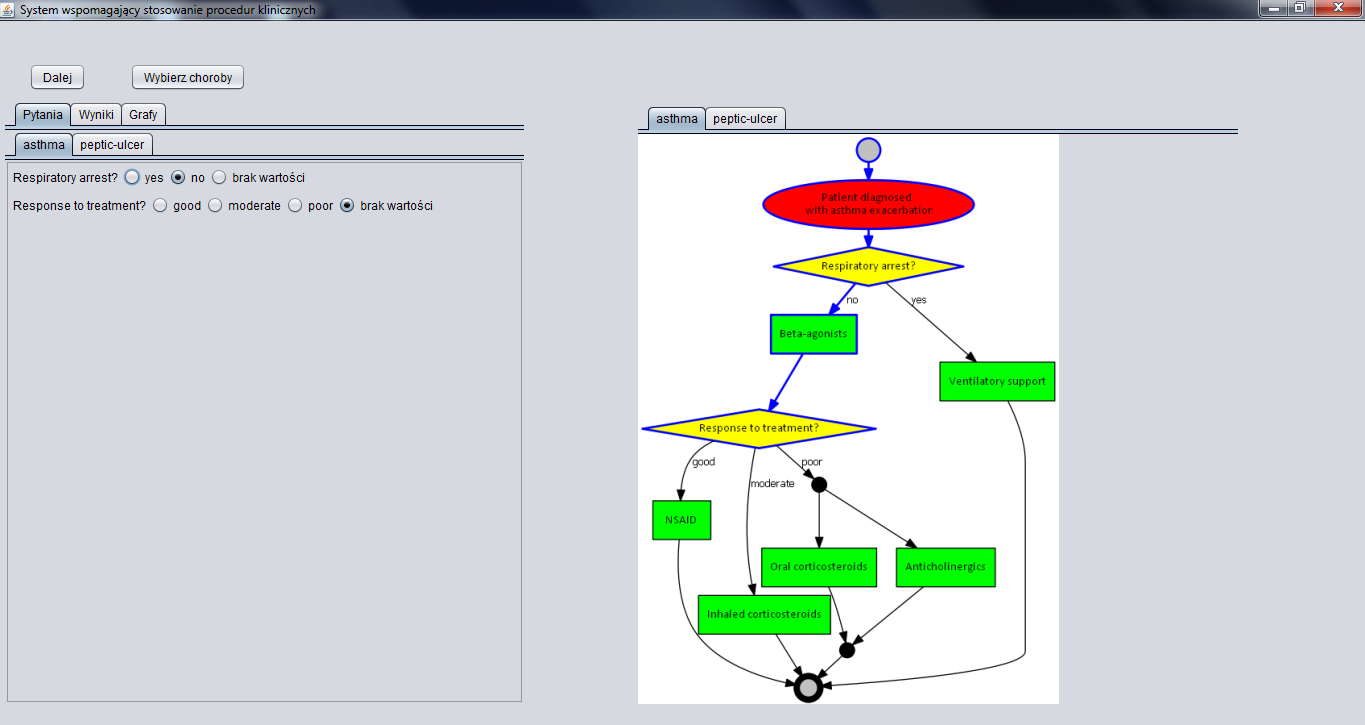
\includegraphics[width=\textwidth]{img/wyswietlanie_grafow.png}
\caption{Wyświetlanie grafów}
\label{fig:wyswietlanie_grafow}
\end{figure}

\section{Udzielanie odpowiedzi na pytania}
% SW2: Biorąc pod uwagę opis, w tym kroku pozwalamy na interakcję z użytkownikiem oraz dokonujemy aktualizacji wyświetlanego grafu. Pojawia się więc pytanie, czym różni się się wyświetlanie grafu po raz pierwszy od kolejnych wyświetleń. Jeśli nie ma różnić (a tak mi się wydaje), to warto połączyć te dwa kroki w jeden (Wyświetlanie i aktualizacja grafów) oraz uprościć ich opis.

Po kliknięciu na jedno z pól wyboru uruchamiana jest procedura \texttt{updateRadioButtonList}. Na początku procedura szuka elementu w liście elementów terapii, którego dotyczy pytanie. Jeśli zaznaczone pole wyboru ma etykietę „brak wartości”, usuwane są wszystkie elementy terapii od elementu, którego dotyczy pytanie, do ostatniego elementu listy. W sytuacji tej cofamy się z udzielaniem odpowiedzi na pytania do jednego z poprzednich pytań.
% SW2: Wyrzuciłbym opis związany z lastNodes -- te szczegóły niczego nie wnoszą.

W kolejnym kroku program ustawia na liście \texttt{lastNodes} węzeł, którego identyfikator jest równy parametrowi question procedury \texttt{updateRadioButtonList}. 
Parametr ten ma wartość równą identyfikatorowi węzła zawierającego pytanie, którego dotyczy zaznaczone pole wyboru. 

% SW2: Ten opis wydaje się niepotrzebnie złożony. Jak rozumiem, działanie programu podczas aktualizacji grafów jest następujące:
% a) po udzieleniu odpowiedzi na wybrane pytanie usuwane są wszystkie elementy terapii znajdujące się po aktualizowanym pytaniu,
% b) jeśli odpowiedź na pytanie jest znana (inna niż "brak danych"), wówczas poruszamy się po grafie, aż dochodzimy do kolejnego kroku decyzyjnego lub liścia w grafie, włączając do terapii wszystkie odwiedzone akcje
% c) jeśli odpowiedź na pytanie jest nieznana ("brak danych"), zatrzymujemy się na aktualizowanym pytaniu

Jeśli natomiast zaznaczone pole wyboru nie posiada etykiety równej „brak wartości” i nie istnieje element na liście elementów terapii, który jest związany z pytaniem, to do tej listy dodawany jest element o wartości równej \texttt{question?answer}, gdzie \texttt{answer} jest parametrem procedury \texttt{updateRadioButtonList} o wartości równej etykiecie krawędzi, z którą jest związane zaznaczone pole wyboru. W sytuacji tej użytkownik udziela po raz pierwszy odpowiedzi na pytanie. 

Jeśli istnieje element związany z pytaniem, to w liście elementów terapii podmieniany jest element, który jest związany z pytaniem na wartość \texttt{question?answer}, a następnie usuwane są wszystkie elementy listy terapii, które się znajdują za podmienionym elementem. 
Następnie pod węzeł o nazwie next podstawiany jest węzeł, który jest pierwszym węzłem krawędzi o etykiecie \texttt{answer} wychodzącej z węzła o identyfikatorze \texttt{question}. 

W kolejnym kroku wywoływana jest procedura \texttt{goForward}, która jako parametr przyjmuje m. in. węzeł \texttt{next}. 
% SW2: Jeśli procedura ta jest wykorzystywana również podczas wyświetlania grafów, to dlaczego Pan o niej nie wspomniał? Połączenie opisów wyświetlania i aktualizacji grafów pozwoli na uniknięcie tego typu problemów.
Procedura ta jest uruchamiana także podczas wyświetlania grafów. Najpierw 
% SW2: Rozumiem, że metoda addToTherapy dodaje aktualny węzeł (n?) do terapii. Jeśli tak, to należy to napisać, aby czytelnik nie musiał się domyślać.
\texttt{goForward} wywołuje metodę \texttt{addToTherapy}, 
% SW2: Co to znaczy, że węzeł n odpowiada węzłowi next? Czy to jeden i ten sam węzeł? Jeśli tak, to lepiej zostać przy jednej zmiennej i nie mnożyć niepotrzebnie bytów.
jeśli węzeł \texttt{n} (odpowiadający węzłowi \texttt{next}) zawiera nie więcej niż jedną krawędź wyjściową lub węzeł \texttt{n} jest węzłem zaczynającym ścieżki równoległe 
% SW2: Poniższy warunek sprawia wrażenie bardzo zawiłego -- w tekście powinno znaleźć się wyjaśnienie, jakiej sytuacji on odpowiada. Przydałaby się też prosta ilustracja graficzna.
i nie jest to węzeł kończący ścieżki równoległe w przypadku, gdy program nie przeszedł jeszcze wszystkich ścieżek równoległych w określonym miejscu. 
% SW: Poniższe sformułowanie może brzmieć dość zaskakująco przy pierwszym czytaniu (odruchowo przyjmuje się, że węzęł kończący ścieżki równoległe nie może być węzłem rozpoczynającym). U nas jest to jednak możliwe -- węzeł parallel może kończyć jeden blok równoległy i ropoczyąć kolejny. Warto dodać taki komentarz, aby recenzent nie miał wątpliwości.
% SW2: Jak już wspomniałem, opis reprezentacji grafu oraz sposób identyfikowania wierzchołków/krokrów powinien pojawić się orzed opisem poszczególnych kroków, aby czytelnik wiedział, czego może oczekiwać. Takie szatkowanie informacji znacznie zmniejsza czytelność tekstu.
Procedura \texttt{addToTherapy}, jeśli etykieta węzła posiada wartość dawki podaną w nawiasach kwadratowych, dodaje do listy elementów terapii identyfikator węzła, po nim znak równości, a następnie wartość dawki. Gdy węzeł nie posiada podanej dawki do listy elementów terapii dodawany jest tylko jego identyfikator. 

% SW2: Czy ta pętla stanowi część metody goForward? Jeśli tak, powinien jawnie Pan to napisać. Co jest celem tej pętli? Przejście tak daleko w "dół" grafu, jak to tylko możliwe?
Następnie program wykonuje pętlę while, której warunek kontynuacji obejmuje 3 przypadki. 
% SW2: Dla każdego z tych warunków powinien Pan podać intuicyjna interpretację oraz ilustrację (np. fragment odpowiedniego grafu).
Pierwszy warunek sprawdza, czy węzeł posiada jedną krawędź wyjściową i nie jest to węzeł kończący ścieżki równoległe chyba, że program zakończył przechodzenie po ścieżkach równoległych związanych z tym węzłem. 
% SW: O tym warunku również była mowa przy okazji metody addToTherapy. Rozumiem, że tutaj jest on sprawdzany dla aktualnego węzła (niekoniecznie n).
% SW2: Te wszystkie informacje o etykietach, krawędziach wchodzących i wychodzących itp. powinni znaleźć się na samym początku przy opisie preprezentacji grafu.
Drugi warunek sprawdza, czy węzeł rozpoczyna ścieżki równoległe, a trzeci czy węzeł kończy ścieżki równoległe. Węzeł rozpoczynający ścieżki równoległe charakteryzuje się tym, że posiada więcej niż jedną krawędź wyjściową oraz nie ma etykiety. Natomiast węzeł kończący ścieżki równoległe posiada więcej niż jedną krawędź wejściową, nie ma etykiety oraz liczba jego krawędzi wyjściowych jest większa od zera. 
Pierwszy warunek jest sprawdzany w kolejnej pętli while, aby dodać do listy elementów terapii wszystkie węzły, które mają tylko jedną krawędź wyjściową, czyli droga, po której należy się poruszać jest jednoznacznie określona. 
Po wykonaniu tej pętli while uzyskujemy węzeł, który jest liściem (nie posiada żadnej krawędzi wyjściowej), 
% SW2: Rozumiem, że oznacza to, że wierzchołek, na którym się zatrzymaliśmy, to liść, krok decyzyjny albo początek klilku równoległych ścieżek, czy tak?
albo ma więcej niż jedną krawędź wyjściową.

W kolejnym kroku sprawdzany jest dla aktualnego węzła drugi warunek w instrukcji if, czyli czy węzeł rozpoczyna ścieżki równoległe. Jeśli jest on spełniony, uzyskany węzeł jest zapisywany do listy węzłów \texttt{parallelNodes}, 
a w liście \texttt{parallelPaths} zapisywana jest liczba 0. 
% SW2: Co rozumie Pan pod pojęciemn "numer krawędzi ścieżek równoległych"? Jak zinterpretować wartość 0? Ponieważ nigdzie później nie wspomina Pan o liście parallelPaths, można usunąć wszelkie informacje o niej, bo bardziej one przeszkadzają, niż pomagają. 
Lista \texttt{parallelPaths} zawiera numer krawędzi ścieżek równoległych, na której aktualnie przebywa program. Później wywoływana jest funkcja \texttt{parallelPath}. 
% SW2: O ile wywołanie parallelPaths dla węzła rozpoczynającego ścieżki równoległe jest intuicyjne (idziemy w głąb grafu), to nie bardzo rozumiem, dlaczego metoda ta jest wywoływana także dla grafu kończącego ścieżki równoległe. To MUSI być wyjaśnione w tekście.
Funkcja ta jest wywoływana również w dla trzeciego przypadku, czyli gdy uzyskany węzeł kończy ścieżki równoległe, a program nie przeszedł jeszcze przez wszystkie te ścieżki. 
% SW2: To jest więcej niż while z 3 warunkami -- tutaj mamy dwie zagnieżdżone pętle. Z jakiej metody pochodzi ten fragnent -- czy z goForward?
Poniższy fragment kodu przedstawia pętlę while z 3 warunkami:

% SW2: Fragment kodu powinien być traktowany jako rysunek lub listing -- powinien mieć swój unikalny numer, a w tekście powinno się znaleźć odwołanie do niego. Poza tym, jeśli zamieszcza Pan fragment kodu, to w tekście (lub w legendzie rysunku) powinno znaleźć się wyjaśnienie wszystkich występujacych tam symboli -- obecnie nie jest jasne, co to jest list i inList oraz dlaczego wierzchołki równoległe mają przypisany identyfikator choroby. Może Pan też na mniej szczegółowy pseudo-kod, ale również wtedy należy się upewnić, że wyjaśnienia są kompletne. Poza tym na listingu warto pokazać numery linii, a następnie odwołać się do nich w opisie.

\newpage
\begin{verbatim}
while((
(list.size()>1)&&(n.getAttribute("label").equals("")))
  ||((inList.size()>1)&& n.getAttribute("label").equals("")
     &&(list.size()>0)&&(parallelNodes.get(idOfDisease)!=null))
  ||((list.size()==1) 
     && (inList.size()<=1 || (inList.size()>1 && !n.getAttribute("label").equals(""))
 	     ||(inList.size()>1 && n.getAttribute("label").equals("")
	        && parallelNodes.get(idOfDisease)==null))))
//warunek1 lub warunek2 lub warunek3
{
    while((list.size()==1) && 
    		(inList.size()<=1 || (inList.size()>1 && !n.getAttribute("label").equals(""))
    		||(inList.size()>1 && n.getAttribute("label").equals("") 
    		   && parallelNodes.get(idOfDisease)==null)))
    //warunek1: węzeł posiada jedną krawędź wyjściową i nie jest to węzeł 
    //kończący ścieżki równoległe chyba, że program zakończył przechodzenie 
    //po ścieżkach równoległych związanych z tym węzłem
    {
    	//dodawanie elementów do terapii i przemieszczanie się 
    	//po grafie do momentu, gdy liczba krawędzi wychodzących jest równa 1
    }
    if((inList.size()>1)&& n.getAttribute("label").equals("")&&(list.size()>0)
        &&(parallelNodes.get(idOfDisease)!=null))
    //warunek2: węzeł kończy ścieżki równoległe
    {
        //wywołanie funkcji parallelPath
    }
    else if((list.size()>1)&&(n.getAttribute("label").equals("")))
    //warunek3: węzeł rozpoczyna ścieżki równoległe
    {
        //wywołanie funkcji parallelPath
    }
}
\end{verbatim}
% SW2: Co rozumie Pan przez "wszystkie ścieżki równoległe"? Wszystkie ścieżki równoległe rozpoczynające się (lub kończące) we wskazanym wierzchołku? To wymaga wyjaśnienia. Nie jest jasne, czy poruszamy się zgodnie kierunkiem krawędzi, czy możemy poruszać się pod prąd. Wreszcie, nie jest jasne, co się stanie w sytuacji, jeśli po wierzchołku kończącym ścieżki równoległe będą same akcje i żadnego pytania? Czy parallelPath kończy działanie także przy osiągnięciu liścia?
Funkcja \texttt{parallelPath} jest w postaci pętli while, która działa dopóki program nie przejdzie przez wszystkie ścieżki równoległe i uzyskany węzeł nie jest węzłem zawierającym pytanie. Pętla while zapisuje do listy elementów terapii wszystkie przebyte po drodze węzły. Na końcu procedura \texttt{goForward} zapisuje do listy węzłów \texttt{lastNodes} uzyskany węzeł, 
% SW2: Również wierzchołki rozpoczynające ścieżki równoległe mogą mieć dwie lub więcej krawędzie wychodzące
jeśli liczba krawędzi wyjściowych węzła jest większa od jeden, czyli jest to węzeł z pytaniem.

Procedura \texttt{updateRadioButtonList} w kolejnym kroku odznacza wszystkie węzły i krawędzie i następnie koloruje je na nowo na podstawie listy elementów terapii. Tworzony jest także nowy obraz grafu za pomocą procedury \texttt{newImageGraph}. Na końcu tworzona jest nowa lista pytań i odpowiedzi za pomocą procedury \texttt{createRadioButtonList}. 
% SW: O jakich przypadkach Pan tutaj mówi? Wszystkich przypadkach modyfikacji danych pacjenta? Tutaj potrzebny jest bardzo precyzyjny opis.


\section{Generowanie terapii}

% SW: Co rozumie Pan przez terapię? Czy jest to ścieżka w grafie reprezentujacym wytyczne? Warto to jawnie zdefniować na samym poczatku opisu. Czy węzeł next to to samo, co węzeł n, który pojawił się poprzednio, czy jest to coś nowego? 
Procedura tworzenia terapii polega na utworzeniu listy terapii zgodnych z odpowiedziami, które zostały udzielone w trakcie zadawania pytań. Na początku procedura szuka węzła, którego identyfikator odpowiada ostatniemu elementowi na liście elementów terapii. Po znalezieniu takiego węzła sprawdzane jest, czy jest to węzeł z pytaniem. Jeśli nie i dodatkowo węzeł nie zawiera krawędzi wyjściowych, zostanie utworzona tylko jedna terapia równa liście elementów terapii. Jeśli natomiast znaleziony węzeł nie posiada pytania i węzeł zawiera krawędzie wyjściowe, do zmiennej next zapisywany jest węzeł występujący bezpośrednio po tym znalezionym. Jeśli z kolei znaleziony węzeł posiada pytanie, do zmiennej next zapisywany jest węzeł, który jest pierwszym węzłem na ścieżce będącej odpowiedzią na pytanie. Odpowiedź na pytanie jest zapisana w elemencie terapii po znaku zapytania.

% SW: Czy dla ścieżek równległych tworzy Pan wiele wersji terapii różnicących się częścią równległą? Jeśli tak, to warto jawnie to wyjaśnić na samym początku opisu.
Później program sprawdza, czy ostatnia udzielona odpowiedź na pytanie znajduje się na równoległej ścieżce. Jeśli tak jest, dla każdej krawędzi wychodzącej z węzła next tworzona jest kopia listy elementów terapii z dodatkowym elementem postaci pytanie?odpowiedź, gdzie pytanie to identyfikator węzła next, a odpowiedź jest etykietą krawędzi wychodzącej z węzła next. 
% SW: Co robi metoda createTherapies?
Następnie program wywołuje funkcję createTherapies. Po wyjściu z pętli program wywołuje funkcję parallelCreateTherapies z parametrem listOfTherapies zawierającym wszystkie terapie uzyskane z wywołań funkcji createTherapies. Jeżeli natomiast pytanie nie znajduje się na równoległej ścieżce, program wywołuje dla każdej jego krawędzi wychodzącej funkcję createTherapies, dodając podobnie jak poprzednio do listy elementów terapii element pytanie?odpowiedź. 

% SW: Opis metody createTherapies powinien znaleźć się tam, gdy odwołuje się Pan do niej po raz pierwszy. Poza tym z opisu wynika, że działa nie metody jest bardzo podobne do updateRadioButtonList. Warto jawnie powiedzieć o tych podobieństwach (i ew. uprościć opis).
Funkcja createTherapies dodaje element terapii odpowiadający pierwszemu węzłowi znajdującemu się na aktualnej ścieżce. Węzeł ten jest dodawany w sytuacji, gdy liczba krawędzi wychodzących z niego jest mniejsza od dwóch lub jest to węzeł rozpoczynający ścieżki równoległe i nie jest to węzeł kończący ścieżki równoległe. Następnie w pętli while dodawane są wszystkie węzły znajdujące się na ścieżce, które posiadają tylko jedną krawędź wychodzącą. Po przejściu przez te węzły program sprawdza, czy uzyskany węzeł jest węzłem końcowym lub węzłem kończącym ścieżki równoległe. W tych sytuacjach funkcja createTherapies zwraca uzyskaną w wyniku dodawania kolejnych węzłów terapię. W przeciwnym razie, jeżeli liczba krawędzi wychodzących z węzła jest większa od jeden i węzeł nie rozpoczyna ścieżek równoległych, czyli jest węzłem z pytaniem, program wywołuje rekurencyjnie dla każdej jego krawędzi wychodzącej funkcję createTherapies. Jeżeli natomiast węzeł rozpoczyna ścieżki równoległe, program wywołuje funkcję parallelCreateTherapies z parameterem listOfTherapies posiadającym jedną, aktualnie tworzoną terapię. 

Funkcja parallelCreateTherapies dla każdej ścieżki wychodzącej z węzła rozpoczynającego ścieżki równoległe przemieszcza się po niej. Podczas poruszania się po ścieżkach program dodaje węzły 
% SW: Tutaj chyba nowe elementy dodawane są tak długo, jak długo liczba krawędzi wychodzących jest równa 1?
do listy elementów terapii do momentu, gdy liczba krawędzi wychodzących z węzła jest równa jeden. Następnie, jeżeli program nie natrafił na węzeł kończący ścieżki równoległe, więc uzyskanym węzłem jest węzeł z pytaniem, dla każdej krawędzi wychodzącej z węzła program wywołuje pętlę for. Pętla ta jest wykonywana dla każdej terapii znajdującej się w liście terapii o nazwie listOfTherapies. 
% SW: Czy metoda createTherapies jest wywoływana ponownie? Bez kodu/pseudo-kodu i przykładów ten opis jest niestety niezrozumiały.
Pętla for wywołuje rekurencyjnie funkcję createTherapies. Uzyskane terapie pobrane z funkcji createTherapies są zapisywane w liście listOfTherapies. Po wykonaniu pętli dla każdej krawędzi wychodzącej z węzła rozpoczynającego ścieżki równoległe, program dla każdej terapii z listOfTherapies wywołuje ponownie funkcję createTherapies. Uzyskane terapie z wszystkich wywołań funkcji createTherapies są zwracane w wyniku funkcji parallelCreateTherapies.

\section{Wyszukiwanie konfliktów}

% SW: Opis tego pliku powinien znaleźć się w osobnej sekcji. Powinien Pan pokazać przykład tego pliku. Wreszcie terminy użyte w poniższym opisie nie są w pełni poprawne -- konflikt to tyle, co niekorzystna interakcja. Po opisie konfliktu następuje opis operacji, jakie należy wykonać, aby zmienić wytyczne i usunąć konflikt.
Program uruchamia procedurę wyszukiwania konfliktów bezpośrednio po utworzeniu terapii. 
% SW: O pliku "nazwy.txt" powinien Pan wspomnieć dopiero przy wyświetlaniu wyników.
Na początku program szuka w katalogu konflikty plików o rozszerzeniu txt oprócz pliku nazwy.txt. Plik nazwy.txt pozwala na nadawanie etykiet elementom dodawanym do grafów wynikowych. Następnie program sprawdza, czy można użyć pliku z konfliktami. Nazwa każdego pliku z konfliktami składa się z listy chorób oddzielonych przecinkami, których dotyczą konflikty. Jeśli jakaś choroba z tej listy znajduje się w wybranych podczas działania programu chorobach, plik zostaje użyty. Każdy plik z konfliktami składa się z linii złożonych z dwóch części. Pierwsza część zawiera elementy, których jednoczesne wystąpienie powoduje wywołanie konfliktu. Elementy te są oddzielone spacją. Druga część linii zawiera interakcje, jakie należy wprowadzić w przypadku zaistnienia konfliktu. Interakcje te są oddzielone od siebie przecinkami. Jeśli plik zostaje użyty, do listy conflictsList dodawane są konflikty, a do listy interactionsList interakcje. 
% SW: Tutaj warto wyjaśnić, że w ten sposób możemy uwzględniać dane pacjenta, które nie wystąpiły jawnie w danych klinicznych.
Ponadto, do listy additionalQuestions dodawane są elementy opisujące konflikt, które rozpoczynają się znakiem „\&”. Dla elementów tych będzie trzeba udzielić odpowiedzi. Elementy konfliktów rozpoczynające się od „not” dodawane są do listy notConflictElems. Następnie program tworzy okienko dialogowe, które pozwala udzielić odpowiedzi na dodatkowe pytania. Pytania mogą być dwóch typów. Pierwszy typ występuje, gdy element nie posiada znaku równości, mniejszości ani większości. Wtedy udzielana odpowiedź ma postać tak/nie. 
% SW: Poniżej powinien pojawić się termin "operator", a nie "znak".
Drugi typ jest typu „zmienna znak liczba”. Znak może być postaci „=”, „>”, „<”, „>=” lub „<=”. Dla tego typu elementu podawana jest wartość liczbowa w okienku dialogowym, a program sprawdza czy podana liczba spełnia warunek występujący w elemencie. 

Po udzieleniu odpowiedzi na wszystkie dodatkowe pytania program przechodzi do kolejnej części wyszukiwania konfliktów o nazwie solveNextPart. Procedura solveNextPart najpierw wywołuje funkcję findSolutions. 
% SW: Skąd biorą się wpisy na liście foundConflicts? Czy są to potencjalne konflikty odczytane z zewnętrznego źródła? Co rozumie Pan przez pojęcie "aktualny konflikt"?
Funkcja ta dla każdego konfliktu wykonuje szereg operacji. Najpierw funkcja sprawdza, czy aktualny konflikt znajduje się na liście foundConflicts. Jeśli konflikt nie znajduje się na tej liście tworzony jest obiekt klasy Solver. Następnie dodawane są zmienne na podstawie wcześniej udzielonych odpowiedzi na dodatkowe pytania. Dokonuje tego procedura setAdditionalVariables. Procedura ta sprawdza, czy pytanie jest typu tak/nie czy odpowiedzią na pytanie jest wartość liczbowa. W pierwszej sytuacji, jeśli odpowiedź jest równa tak, program tworzy zmienną biblioteki Choco typu IntVar o wartości równej jeden. Jeżeli odpowiedź jest równa nie, program tworzy zmienną IntVar o wartości równej zero. Jeśli odpowiedzią na pytanie jest wartość liczbowa, program tworzy zmienną IntVar o wartości równej podanej liczbie. Każda z utworzonych zmiennych jest dodawana do globalnej listy addedVarsList, która jest tworzona na początku procedury. 

Po wykonaniu procedury setAdditionalVariables program wywołuje procedurę setVariables. 
% SW: Co przechowują listy therapiesList oraz globalConflictsList? Ponadto z opisu wynika, że therapiesList oraz lista terapii przechowują tę samą informację. 
Procedura ta najpierw tworzy globalne listy therapiesList oraz globalConflictsList. Następnie dla każdej choroby tworzona jest tablica terapii. W kolejnym kroku dla każdej terapii choroby tworzona jest zmienna IntVar 
% SW: Do czego służy ta zmienna?
o nazwie „choroba\_terapiaX”, gdzie choroba jest nazwą choroby, a X jest numerem terapii. Zmienna ta przyjmuje wartości zero lub jeden. Zmienna jest zapisywana w tablicy terapii i dodawana do listy therapiesList. 
% SW: Czy dla każdej terapii/ścieżki tworzona jest osobna lista notConflictsElemsTherapy?
Następnie program tworzy listę notConflictElemsTherapy, do której dodawane są te elementy konfliktu z listy notConflictElems, które nie znajdują się na liście elementów konkretnej terapii, ale znajdują się w grafie związanym z terapią. Elementy listy notConflictElemsTherapy są unikalne, nie powtarzają się. Następnie program tworzy tablicę vars, która będzie zawierała zmienne wchodzące w skład pojedynczej terapii. W kolejnym kroku dla każdego elementu listy notConflictElemsTherapy szukana jest zmienna 
% SW: Nigdzie nie wyjaśnił Pan, do czego służy ta lista? Opis procedury powinien rozpocząć Pan od przedstawienia i omówienia istotnych struktur danych. Poza tym powinien przedstawić Pan ogólną zasadę tworzenia zmiennych (i zilustrować ją przykładem) -- natychmiastowe zejście na poziom szczegółowego opisu implementacji powoduje, że staje się on zupełnie nieczytelny. 
w addedVarsList, której nazwa odpowiada elementowi listy. Jeśli taka zmienna istnieje, zapisywana jest w zmiennej medicineVar. Jeśli natomiast nie istnieje, jest tworzona i dodawana do addedVarsList. Następnie program szuka zmiennej w addedVarsList o nazwie „not\_X”, gdzie X jest elementem terapii. Jeśli taka zmienna istnieje, zapisywana jest w zmiennej notMedicineVar. Jeśli natomiast nie istnieje, do zmiennej notMedicineVar zapisywana jest nowo tworzona zmienna, której wartość jest równa 0, gdy medicineVar jest równa 1 i odwrotnie. Następnie zmienna notMedicineVar jest zapisywana do listy addedVarsList. W kolejnym kroku zmienna notMedicineVar jest zapisywana w tablicy vars. Ponadto, dla każdego elementu terapii program zapisuje do zmiennej medicineName nazwę elementu terapii. Następnie program szuka zmiennej odpowiadającej elementowi terapii w liście addedVarsList. Jeśli występuje w tej liście szukana zmienna, program zapisuje ją w zmiennej medicineVar i tworzy dodatkowo zmienną „X\_dosage”, gdzie X jest elementem terapii. Program dodaje zmienną „X\_dosage” w sytuacji, gdy element terapii posiada dawkę i zmienna nie występuje w addedVarsList. Jeśli szukana zmienna nie została odnaleziona, program tworzy zmienną IntVar zero-jedynkową o nazwie równej medicineName i dodaje ją do listy addedVarsList. Jeśli dodatkowo element terapii zawiera dawkę, oprócz zmiennej zero-jedynkowej tworzona jest zmienna IntVar o nazwie będącej połączeniem medicineName i „\_dosage”. Wartość tej zmiennej odpowiada wartości zapisanej w elemencie terapii. Następnie program dodaje ograniczenie polegające na tym, że zmienna „choroba\_terapiaX” przyjmuje wartość jeden, gdy suma zmiennych należących do tablicy vars jest równa wielkości tej tablicy. Wartość zero przyjmuje zmienna terapii w przeciwnym razie. Po przejściu przez wszystkie terapie określonej choroby program dodaje ograniczenie polegające na tym, że suma zmiennych terapii choroby ma być równa jeden, czyli dla każdej choroby ma zostać użyta tylko jedna terapia. 

% SW: Tutaj przestałem czytać -- bez przykładów, pseudokodu oraz (przede wszystkim) wysokopoziomowego opisu tego, co chce Pan osiągnąć oraz dlaczego, ten tekst jest nieczytelny i recenzent (podobnie jak ja) na nim padnie.
Po wykonaniu procedury setVariables program dodaje ograniczenia konfliktów. Najpierw dodawane są ograniczenia tych konfliktów, które występowały w poprzednich iteracjach pętli for i po których dodaniu zostało wygenerowane poprawne rozwiązanie. Następnie dodawane jest ograniczenie konfliktu, które odpowiada aktualnej iteracji pętli. Procedura dodawania ograniczeń konfliktu ma nazwę setConflictConstraint. Procedura ta najpierw tworzy listę o nazwie constraintsList. Następnie procedura wywołuje pętlę for dla każdego elementu wchodzącego w skład konfliktu. Pętla ta najpierw sprawdza czy element konfliktu zawiera znak równości, mniejszości lub większości i nie zawiera znaku zapytania. Jeśli tak nie jest, ale element konfliktu rozpoczyna się od operatora „not”, program szuka zmiennej zawartej w not w addedVarsList. Jeśli taka zmienna istnieje, program dodaje ograniczenie „not(zmienna=1)” do listy constraintsList. Jeśli natomiast program nie znalazł zmiennej, jest ona tworzona, jest dodawane dla niej ograniczenie „not(zmienna=1)” oraz zmienna dodawana jest do addedVarsList. W obu sytuacjach program dodaje zmienne do globalConflictsList. Jeśli element konfliktu nie zawiera znaku równości, mniejszości ani większości i nie rozpoczyna się od „not”, program sprawdza, czy istnieje zmienna w addedVarsList o nazwie równej elementowi konfliktu. Dla tej sytuacji procedura dodaje ograniczenie postaci „zmienna=1” do listy constraintsList oraz nazwę zmiennej do listy globalConflictsList. Jeśli nie istnieje zmienna w addedVarsList, program tworzy nową zmienną IntVar, dodaje ograniczenie „zmienna=1” do listy constraintsList, nazwę nowej zmiennej do globalConflictsList oraz zmienną do addedVarsList. Jeżeli natomiast element konfliktu zawiera znak równości, mniejszości lub większości i nie zawiera znaku zapytania, procedura wywołuje metodę o nazwie conflictWithDosage. Metoda ta szuka zmiennej w addedVarsList, której nazwa jest równa nazwie elementu konfliktu. Jeśli istnieje taka zmienna i nazwa zmiennej rozpoczyna się od „\&”, dodawane jest ograniczenie postaci „zmienna znak wartość” do listy constraintsList oraz dodawana jest nazwa zmiennej do listy globalConflictsList. Jeśli znaleziono odpowiednią zmienną, ale jej nazwa nie rozpoczyna się od „\&”, dodawane są dwa ograniczenia do constraintsList. Pierwsze ograniczenie jest postaci „zmienna=1”, drugie natomiast jest postaci „zmienna\_dosage znak wartość”. Oba te ograniczenia są dodawane do listy constraintsList oraz ich nazwy są dodawane do listy globalConflictsList. Jeśli program nie znalazł w addedVarsList zmiennej, której nazwa równa jest nazwie elementu konfliktu,  tworzy zmienną IntVar o nazwie „zmienna\_false”. Ograniczenie „zmienna\_false=0” jest również dodawane do listy constraintsList oraz nazwa zmiennej jest dodawana do globalConflictsList. Po wykonaniu pętli dla każdego elementu konfliktu procedura tworzy z listy constraintsList tablicę, a następnie dodaje do solvera ograniczenie postaci not(and(ograniczenia)). 

Po wykonaniu procedury setConflictConstraint program wykonuje procedurę addConstraintsTrue, która dla każdej zmiennej w addedVarsList, która nie istnieje na liście globalConflictsList i nie rozpoczyna się od „\&” ani nie kończy się na „\_dosage”, dodaje ograniczenie do solvera postaci „zmienna=1”. Po wykonaniu procedury addConstraintsTrue program wywołuje metodę findSolution obiektu klasy Solver, które dokonuje znalezienie rozwiązania problemu. Jeśli rozwiązanie istnieje, do avoidedConflicts dodawany jest numer konfliktu na liście conflictsList. Jeśli natomiast nie ma rozwiązania, do foundConflicts dodawany jest konflikt oraz do interactionsList dodawane są interakcje odpowiadające konfliktowi. Ponadto, gdy nie ma rozwiązania program wywołuje procedurę executeInteractions, która dokonuje zmian w terapiach, a także program wywołuje rekurencyjnie funkcję findSolutions, aby sprawdzić, czy wprowadzone zmiany nie spowodowały wystąpienia konfliktów, dla których już dokonało się przeglądu, oraz aby sprawdzić kolejne konflikty. Po wywołaniu funkcji findSolutions program ustawia wartość stop na true, co powoduje, że program nie sprawdza wystąpienia kolejnych konfliktów, ponieważ zrobiła już to wywołana rekurencyjnie funkcja findSolutions. 

Ostatecznie, program dokonuje rozwiązania problemu z tymi ograniczeniami w postaci konfliktów, które znajdują się na liście avoidedConflicts. Po wygenerowaniu pierwszego rozwiązania program tworzy listę o nazwie solutions. Następnie w pętli do/while, która działa dopóki istnieje kolejne rozwiązanie, program zapisuje do zmiennej solution po przecinku nazwy zmiennych terapii, które posiadają wartość równą jeden. Następnie, jeśli zmienna solution nie znajduje się jeszcze w liście solutions, zmienna dodawana jest do tej listy. Na końcu program do listy therapies dodaje rozwiązania. Polega to na tym, że dla każdego elementu listy solutions o nazwie elem program tworzy listę o nazwie therapiesSolution. Następnie tworzy tablicę zawierającą elementy, które były w zmiennej elem rozdzielone przecinkami. W kolejnym kroku dla każdej choroby znajdującej się w liście diseases szuka elementu w tablicy, którego nazwa rozpoczyna się od nazwy choroby. Następnie do listy therapiesSolution dodaje listę z therapiesDiseases o numerze równym numerowi choroby i podnumerze równym X znajdującym się w nazwie zmiennej terapii „choroba\_terapiaX”. Na końcu program wywołuje procedurę setResults, która pozwala na zaprezentowanie wyników. 

\section{Wyświetlanie wyników}

Program prezentuje wyniki za pomocą procedury setResults. Na początku procedura wywołuje inną procedurę o nazwie setGraphs. Zajmuje się ona wyświetleniem wyników w postaci grafów. Najpierw procedura usuwa wszystkie zakładki z rozwiązaniami z zakładki „Grafy”. W kolejnym kroku wywołuje dwie pętle, z których druga się zawiera w pierwszej. Pierwsza pętla porusza się po rozwiązaniach, druga po terapiach pojedynczego rozwiązania. Dla każdej terapii, która jest związana z określoną chorobą, tworzony jest odpowiedni graf. Następnie procedura wywołuje pętlę po grupach interakcji poszczególnych konfliktów oraz po pojedynczych interakcjach. 
% SW: To nie są interakcje, ale operacje modyfikujące wytyczne. Poza tym modyfikacja wytycznych powinna być omówiona jako osobny punkt ("Usuwanie konfliktów") -- tam właśnie powinna się znaleźć duża część poniższego tekstu. Pza tym również tutaj warto byłoby pokazać przykład realizacji poszczególnych typów operacji. 

Dla każdej interakcji sprawdzany jest jej typ. Interakcje mogą być kilku typów. Pierwszy typ to „replace X with Y”, który polega na tym, że węzeł X zamienia się na węzeł Y. Kolejny typ to „add X before/after Y”, który charakteryzuje się tym, że węzeł X jest dodawany przed lub po elemencie Y w zależności od tego, czy zostało użyte before czy after. Kolejnym typem jest „remove X”, które polega na usunięciu węzła X. Istnieją jeszcze typy interakcji postaci „increase\_dosage X Y”, „decrease\_dosage X Y”, które powodują zwiększenie lub zmniejszenie dawki węzła X o Y. Ostatnim typem jest „change\_dosage X Y”, które polega na zmianie dawki węzła X na wartość Y.  

Jeśli interakcja jest typu „replace”, najpierw program szuka węzła o identyfikatorze równym elementowi, który należy zamienić. Po znalezieniu takiego węzła z pliku nazwy.txt odczytywana jest etykieta elementu, który ma się znaleźć na miejscu zamienianego elementu. Etykieta jest następnie zapisywana jako etykieta znalezionego węzła. Ponadto, program zamienia identyfikator znalezionego węzła na nowy. Jeśli interakcja jest typu „add”, program szuka węzła, przed lub za którym ma zostać umieszczony nowy węzeł. Następnie program tworzy nowy węzeł, nadaje mu etykietę pobraną z pliku nazwy.txt i dodaje węzeł do grafu. Następnie, jeżeli element, względem którego ma zostać wstawiony nowy węzeł jest postaci „pytanie?odpowiedź”, dla krawędzi, która ma etykietę „odpowiedź”, program ustawia węzeł docelowy krawędzi na nowo utworzony węzeł. Następnie, program tworzy nową krawędź, której węzłem źródłowym jest nowo utworzony węzeł, a węzłem docelowym jest węzeł docelowy krawędzi o etykiecie „odpowiedź”. Powoduje to umieszczenie nowego węzła na początku krawędzi z etykietą „odpowiedź”. Jeżeli natomiast element, względem którego ma być wstawiony nowy węzeł nie jest typu „pytanie?odpowiedź”, mogą wystąpić dwa przypadki. Pierwszy przypadek występuje, gdy interakcja jest typu „add X after Y”, drugi, gdy interakcja jest typu „add X before Y”. Dla tych sytuacji nowy węzeł jest umieszczany odpowiednio za lub przed węzłem Y. 

W przypadku, gdy typ interakcji to „remove”, program przypisuje znalezionemu węzłowi atrybut style na wartość „invis”, atrybut fixedsize na „true” oraz atrybuty height i width na „0”. Powoduje to, że węzeł usunięty staje się niewidoczny na tworzonym grafie. Dla typów interakcji „increase\_dosage”, „decrease\_dosage” i „change\_dosage” odpowiednio zmienia się końcową część etykiety z nawiasami kwadratowymi, która przedstawia dawkę. Na końcu procedura setGraphs dla każdego grafu wywołuje procedurę color zaznaczającą przebyte węzły i krawędzie, a następnie procedurę newImageGraph, która powoduje wygenerowanie grafu w postaci obrazkowej. 

Po wywołaniu procedury setGraphs program tworzy rozwiązania tekstowe. Polega to na utworzeniu dla każdego rozwiązania i dla każdej choroby pojedynczego rozwiązania dwóch pól tekstowych. Pierwsze z nich przedstawia etykiety przebytych węzłów, a drugie ich identyfikatory. 
% SW: Poniższe zdanie jest nadmiarowe -- wynika z niego, że etykietę węzła otrzymuje się odczytując etykietę węzła... Raczej należałoby się skupić na tym, że w przypadku węzłów decyzyjnych łączymy etykietę węzła z etykietą wybranej krawędzi.
Etykietę węzła otrzymuje się przez znalezienie węzła o identyfikatorze równym elementowi terapii, a następnie odczytanie jego etykiety. Dla węzła pytającego program wypisuje dodatkowo etykietę wybranej krawędzi. Jeśli jest taka potrzeba, program szuka etykiety węzła w pliku nazwy.txt. Drugie pole tekstowe, z identyfikatorami, program tworzy wypisując elementy terapii z listy. Elementy są oddzielone od siebie znakiem nowej linii. 
% SW: Tutaj również powinien pokazać przykładowy ekran i wskazań na nim elementy, o których Pan wspomina w opisie.
Po utworzeniu pól tekstowych program umieszcza je na panelu, który jest z kolei umieszczany na zakładce. Na końcu program wypisuje w odpowiednim polu tekstowym konflikty i związane z nimi interakcje. Podczas wypisywania konfliktów i interakcji program szuka odpowiednich etykiet węzłów w grafie lub w pliku nazwy.txt. 

